%%%%%%%%%%%%%%%%%%%%%%%%%%%%%%%%%%%%%%%%%
% Classicthesis Typographic Thesis
% LaTeX Template
% Version 1.4 (1/1/16)
%
% This template has been downloaded from:
% http://www.LaTeXTemplates.com
%
% Original author:
% André Miede (http://www.miede.de) with commenting modifications by:
% Vel (vel@LaTeXTemplates.com)
%
% License:
% GNU General Public License (v2)
%
% General Tips:
% 1) Make sure to edit the classicthesis-config.file
% 2) New enumeration (A., B., C., etc in small caps): \begin{aenumerate} \end{aenumerate}
% 3) For margin notes: \marginpar or \graffito{}
% 4) Do not use bold fonts in this style, it is designed around them
% 5) Use tables as in the examples
% 6) See classicthesis-preamble.sty for useful commands
%
%%%%%%%%%%%%%%%%%%%%%%%%%%%%%%%%%%%%%%%%%

%----------------------------------------------------------------------------------------
%	SILENCE ANNOYING WARNINGS
%----------------------------------------------------------------------------------------

\RequirePackage{silence}
\WarningFilter{titlesec}{Non standard sectioning command}
\WarningFilter{scrreprt}{Usage of package}
\WarningFilter{scrreprt}{Activating an ugly workaround}
\WarningFilter{titlesec}{Non standard sectioning command detected}


% **************************************************
% Document Class Definition
% **************************************************
\documentclass[%
	paper=A4,					% paper size --> A4 is default in Germany
	twoside=true,				% onesite or twoside printing
	openright,					% doublepage cleaning ends up right side
	parskip=full,				% spacing value / method for paragraphs
	chapterprefix=true,			% prefix for chapter marks
	11pt,						% font size
	headings=normal,			% size of headings
	bibliography=totoc,			% include bib in toc
	listof=totoc,				% include listof entries in toc
	titlepage=on,				% own page for each title page
	captions=tableabove,		% display table captions above the float env
	draft=false,				% value for draft version
    openany						% Avoid blank page after each new part, chapter, ...
]{scrreprt}%

%%%%%%%%%%%%%%%%%%%%%%%%%%%%%%%%%%%%%%%%%
% Thesis Configuration File
%
% This file has been downloaded from:
% http://www.LaTeXTemplates.com
%
% Original author:
% André Miede (http://www.miede.de) with extensive commenting changes by:
% Vel (vel@LaTeXTemplates.com)
%
% License:
% GNU General Public License (v2)
%
% Important note:
% The main lines to change in this file are in the DOCUMENT VARIABLES
% section, the rest of the file is for advanced configuration.
%
%%%%%%%%%%%%%%%%%%%%%%%%%%%%%%%%%%%%%%%%%

\usepackage[utf8]{inputenc}		% defines file's character encoding

\usepackage[french,main=french]{babel} % babel system, adjust the language of the content

\usepackage[					% clean thesis style
	figuresep=colon,%
	sansserif=true,%
	hangfigurecaption=false,%
	hangsection=true,%
	hangsubsection=true,%
	colorize=full,%
	colortheme=bluegreen,%
% LLT: Use biber if using UTF8 encoding
% 	bibsys=bibtex,%
	bibsys=biber,%
% 	bibfile=bib-refs,%
    bibfile=library,%
	bibstyle=numeric,%
%     bibstyle=apa,%
]{cleanthesis}

% **************************************************
% DOCUMENT VARIABLES
% **************************************************
% \newcommand{\thesisTitle}{D\'eveloppement de nouvelles strat\'egies de pr\' ediction structurale à partir de contacts \'evolutifs\xspace}
\newcommand{\thesisTitle}{Comment la protéine prion PrP\up C est impliquée dans l'inflammation pulmonaire chronique?\\ Rôle de l'homéostasie du cuivre et du stress oxydatif\xspace}
\newcommand{\thesisName}{Amal Kouadri\xspace}
\newcommand{\thesisSubject}{Thèse de doctorat en Sciences de la Vie\xspace}
\newcommand{\thesisDate}{Automne 2017}
\newcommand{\thesisVersion}{0.1}

\newcommand{\thesisFirstReviewer}{Jane Doe}
\newcommand{\thesisFirstReviewerUniversity}{\protect{Clean Thesis Style University}}
\newcommand{\thesisFirstReviewerDepartment}{Department of Clean Thesis Style}

\newcommand{\thesisSecondReviewer}{John Doe}
\newcommand{\thesisSecondReviewerUniversity}{\protect{Clean Thesis Style University}}
\newcommand{\thesisSecondReviewerDepartment}{Department of Clean Thesis Style}

\newcommand{\thesisFirstSupervisor}{Dr. Mohamed BENHAROUGA}
\newcommand{\thesisSecondSupervisor}{}

\newcommand{\thesisUniversity}{\protect{Université Grenoble Alpes}}
\newcommand{\thesisUniversityDepartment}{\'Ecole doctorale Chimie et Sciences du vivant}
\newcommand{\thesisUniversityInstitute}{CEA Grenoble}
\newcommand{\thesisUniversityGroup}{Laboratoire de Chimie et Biologie des Métaux (LCBM)\\ \'Equipe Biologie des Métaux (BioMet)}
\newcommand{\thesisUniversityCity}{Grenoble}
\newcommand{\thesisUniversityStreetAddress}{17 rue des martyrs}
\newcommand{\thesisUniversityPostalCode}{38000}

%----------------------------------------------------------------------------------------
%	USEFUL COMMANDS
%----------------------------------------------------------------------------------------

\newcommand{\ie}{i.\,e.}
\newcommand{\Ie}{I.\,e.}
\newcommand{\eg}{e.\,g.}
\newcommand{\Eg}{E.\,g.} 

\newcounter{dummy} % Necessary for correct hyperlinks (to index, bib, etc.)
\providecommand{\mLyX}{L\kern-.1667em\lower.25em\hbox{Y}\kern-.125emX\@}
\newlength{\abcd} % for ab..z string length calculation

% **************************************************
% Load and Configure Packages
% **************************************************

\hypersetup{					% setup the hyperref-package options
	pdftitle={\thesisTitle},	% 	- title (PDF meta)
	pdfsubject={\thesisSubject},% 	- subject (PDF meta)
	pdfauthor={\thesisName},	% 	- author (PDF meta)
	plainpages=false,			% 	-
	colorlinks=true,			% 	- colorize links?
    linktocpage=true,
	pdfborder={0 0 0},			% 	-
	breaklinks=true,			% 	- allow line break inside links
	bookmarksnumbered=true,		%
	bookmarksopen=true,			%,
    linkcolor=ctcolorblue,
    citecolor=black,
}

\PassOptionsToPackage{acronym,translate=babel,xindy,toc,nopostdot,nonumberlist}{glossaries}
\usepackage{glossaries}

\usepackage{chngcntr}			% Reset Chapter counter for each part
\counterwithin*{chapter}{part}

\DeclareCiteCommand{\citeauthorfirstlast}
  {\boolfalse{citetracker}%
   \boolfalse{pagetracker}%
   \DeclareNameAlias{labelname}{first-last}%
   \usebibmacro{prenote}}
  {\ifciteindex
     {\indexnames{labelname}}
     {}%
   \printnames{labelname}}
  {\multicitedelim}
  {\usebibmacro{postnote}}


% **************************************************
% Debug LaTeX Information
% **************************************************
%\listfiles
%----------------------------------------------------------------------------------------
%	Glossary
%----------------------------------------------------------------------------------------
\newglossaryentry{recuit}{
    name={recuit simulé},
    description={Protocole de recherche de la forme la plus stable du système étudié. Cette forme est dans ce casElle de plus basse énergie correspondant à la recherche du minimum global de la surface d'énergie potentielle du système moléculaire. Cette méthode a une phase de simulation à haute température permettant d'explorer l'espace conformationnel et une deuxième de refroidissement pour atteindre un autre minimum local ou global du système.}
}
\newglossaryentry{coupscal}{
    name={couplage scalaire},
    description={Interaction correspondant à un transfert d'aimantation entre deux noyaux séparés par une ou plusieurs liaisons covalentes. La force est mesurée par les constantes de couplage qui dépendent du type des noyaux impliqués.}
}
\newglossaryentry{coupdip}{
    name={couplage dipolaire},
    description={Association entre deux noyaux proches dans l'espace. Le transfert d'aimantation observés entre les deux noyaux est affecté par les mouvements browniens en solution. Cet effet est communément nommé  dans cette situation l'effet Overhauser nucléaire (\acrshort{noe}).},
    plural={couplages dipolaires}
}
\newglossaryentry{cdr}{
    name={contrainte de distance ambiguë},
    description={Chaque pic croisé d'un spectre \acrshort{noesy} est traité comme étant la superposition des signaux  des assignations possibles du pic. Les contraintes calculées (Distance effective $R$) sont proportionnelles à la somme de l'inverse des distances interatomiques élevées ($r$) à la puissance 6 de chaque assignation possible. \begin{equation}\frac{1}{R^6} = \sum_{i}^{n}\frac{1}{r_{i}^6}\end{equation}}
}
\newglossaryentry{rdc}{
    name={couplage dipolaire résiduel},
    description={Dans le cas d'expérimentations \acrshortpl{rmn} dans des milieux partiellements orientés, des couplages dipolaires résiduels sont mesurés et leur valeur est proportionnelle à $\frac{1}{r^3}$ ($r$ est la distance inter-atomique) mais dépend également des angles $\theta$ entre les liaisons covalentes et le vecteur du champ magnétique statique. }
}
\newglossaryentry{apidef}{
    name={interface de programmation (API)},
    description={Regroupe l'ensemble des classes, méthodes et fonctions d'une application souvent stockés dans une bibliothèque logicielle et qui permettent aux autres logiciels d'avoir accès aux différentes fonctionnalités de l'application. Elle correspond par exemple aux classes d'ARIA sauvegardant les paramètres.}
}
\newglossaryentry{framew}{
    name={framework},
    description={Ensemble cohérent de composants logiciels permettant de définir les bases d'une application. Il définit un environnement de travail au développeur proposant un ensemble d'outils et guide l'architecture du futur logiciel.}
}
\newglossaryentry{ormdef}{
    name={mapping objet relationnel (ORM)},
    description={Concept de programmation permettant de convertir un ensemble d'objets en une base de données relationnelle.}
}

%----------------------------------------------------------------------------------------
%	Acronyms
%----------------------------------------------------------------------------------------
\newacronym{xml}{XML}{Extensible Markup Language}
\newacronym{noesy}{NOESY}{Spectroscopie d'Effet Overhauser Nucleaire}
\newacronym{aria}{ARIA}{Ambiguous Restraints for Iterative Assignment}
\newacronym{rmn}{RMN}{Résonance Magnétique Nucléaire}
\newacronym{cns}{CNS}{Crystallography \& NMR System}
\newacronym{mtf}{MTF}{Molecular Topology File}
\newacronym{noe}{NOE}{Effet Overhauser Nucléaire}
\newacronym{embl}{EMBL}{European Molecular Biology Laboratory}
\newacronym{bis}{BIS}{Bioinformatique Structurale}
\newacronym{wenmr}{WeNMR}{Worldwide e-Infrastructure for NMR and structural biology}
\newacronym{api}{API}{Interface de Programmation (Application Programming Interface)}
\newacronym{cib}{CIB}{Centre d'Informatique pour la Biologie}
\newacronym{ccpn}{CCPN}{Collaborative Computing Project for the NMR community}
\newacronym{pdb}{PDB}{Protein Data Bank}
\newacronym{mtv}{MTV}{Modèle Template Vue}
\newacronym{mvc}{MVC}{Modèle Vue Contrôleur}
\newacronym{html}{HTML}{Hypertext Markup Language}
\newacronym{orm}{ORM}{Mapping Objet Relationnel}
\newacronym{rmsd}{RMSD}{Root Mean Square Deviation}
\newacronym{dry}{DRY}{Don't Repeat Yourself}
\newacronym{cgi}{CGI}{Common Gateway Interface}
\newacronym{casd}{CASD-NMR}{Critical Assessment of Automated Structure Determination of Proteins from NMR Data}
\makeglossaries

% **************************************************
% Document CONTENT
% **************************************************
\begin{document}

%----------------------------------------------------------------------------------------
%	PRE-CONTENT THESIS PAGES
%----------------------------------------------------------------------------------------

% \frenchspacing % Reduces space after periods to make text more compact

% \raggedbottom % Makes all pages the height of the text on that page

\pagenumbering{roman} % Roman page numbering prior to the start of the thesis content (i, ii, iii, etc)
\pagestyle{empty} % Suppress headers for the pre-content pages

% !TEX root = ../thesis-example.tex
%
% ------------------------------------  --> cover title page
\begin{titlepage}
	\pdfbookmark[0]{Cover}{Cover}
	\flushright
	\hfill
	\vfill
	{\LARGE\thesisTitle \par}
	\rule[5pt]{\textwidth}{.4pt} \par
	{\Large\thesisName}
	\vfill
	\textit{\large\thesisDate} \\
	Version: \thesisVersion
\end{titlepage}


% ------------------------------------  --> main title page
\begin{titlepage}
	\pdfbookmark[0]{Titlepage}{Titlepage}
	\tgherosfont
	\centering

	{\Huge \thesisUniversity} \\[2mm]
    {\Large \thesisUniversityDepartment} \\[4mm]
	
\includegraphics[width=6cm]{gfx/logo-uga.png} \\[2mm]
	
	\textsf{\large \thesisUniversityGroup} \\
    \textsf{\large \thesisUniversityInstitute} \\

	\vfill
	{\Large \thesisSubject} \\[5mm]
	{\LARGE \color{ctcolortitle}\textbf{\thesisTitle} \\[10mm]}
	{\Large \thesisName} \\

	\vfill
	\begin{minipage}[t]{.27\textwidth}
		\raggedleft
		\textit{1. Reviewer}
	\end{minipage}
	\hspace*{15pt}
	\begin{minipage}[t]{.65\textwidth}
		{\Large \thesisFirstReviewer} \\
	  	{\small \thesisFirstReviewerDepartment} \\[-1mm]
		{\small \thesisFirstReviewerUniversity}
	\end{minipage} \\[5mm]
	\begin{minipage}[t]{.27\textwidth}
		\raggedleft
		\textit{2. Reviewer}
	\end{minipage}
	\hspace*{15pt}
	\begin{minipage}[t]{.65\textwidth}
		{\Large \thesisSecondReviewer} \\
	  	{\small \thesisSecondReviewerDepartment} \\[-1mm]
		{\small \thesisSecondReviewerUniversity}
	\end{minipage} \\[10mm]
	\begin{minipage}[t]{.27\textwidth}
		\raggedleft
		\textit{Encadrants}
	\end{minipage}
	\hspace*{15pt}
	\begin{minipage}[t]{.65\textwidth}
		\thesisFirstSupervisor\ et \thesisSecondSupervisor
	\end{minipage} \\[10mm]

	\thesisDate \\
    \vfill
    


\end{titlepage}


% ------------------------------------  --> lower title back for single page layout
\hfill
\vfill
{
	\small
	\textit{\thesisTitle,} \thesisName \\
    \textcopyright\ \thesisDate \\
	\thesisSubject\\
	Rapporteurs: \thesisFirstReviewer\ and \thesisSecondReviewer \\
	Directeur de th\`ese: \thesisFirstSupervisor\\
	\textbf{\thesisUniversity} \\
	\thesisUniversityDepartment \\
    \textit{\thesisUniversityGroup} \\
	\thesisUniversityInstitute \\
	\thesisUniversityStreetAddress \\
	\thesisUniversityPostalCode\ \thesisUniversityCity
}
		% INCLUDE: all titlepages

\pagestyle{plain}				% display just page numbers

\clearpage% !TEX root = ../thesis-example.tex
%
\pdfbookmark[0]{\abstractname}{\abstractname}

\begingroup

\let\clearpage\relax
\let\cleardoublepage\relax
\let\cleardoublepage\relax

\chapter*{\abstractname}\label{sec:abstract}
\vspace*{-10mm}

Dans la fibrose kystique (FC), l'inflammation est détectée au début de la voie aérienne, même avant le début de l'infection bactérienne. Cela suggère que les mécanismes autres que l'infection sont à l'origine du processus initial d'inflammation. Parmi ces processus, il y a le stress oxydatif. Ce dernier est largement reconnu comme un élément essentiel de plusieurs maladies.
Récemment, nous avons observé que les cellules et les tissus des patients bronchiques des FC présentent une augmentation de la concentration de Cu, dans la production de radicaux libres, dans les activités enzymatiques pro et antioxydantes, et une diminution de la concentration de glutathion, un chelate naturel de Cu intracellulaire. Ces résultats et d'autres nous ont permis d'établir le lien avec Cu, le stress oxydatif, l'inflammation et l'infection.
En étudiant le niveau d'expression d'un certain nombre de gènes codant pour les protéines de l'homéostasie du Cu, nous avons constaté que l'expression de la protéine prion cellulaire (PrPC) a été modifiée. PrPC est une glycoprotéine chantée de glycosyl phosphatidyl inositol (GPI) qui a été impliquée dans la propagation et l'agrégation des prions dans le système nerveux central qui conduit à des maladies des encéphalopathies spongiformes transmissibles (EST).
Cependant, en dépit de plusieurs études in vitro et in vivo qui ont démontré la capacité de PrPC à interagir avec d'autres protéines, à lier le cuivre (Cu) avec une affinité élevée et à protéger les cellules contre le stress oxydatif, ses fonctions physiologiques sont encore à l'étude, en particulier dans Des tissus extra-neuronaux, tels que l'épithélium bronchique.
Dans le présent projet, nous avons étudié le rôle de PrPC dans l'architecture cellulaire pulmonaire en déterminant son impact sur l'intégrité des jonctions épithéliales pulmonaires par rapport à l'inflammation, l'homéostasie du Cu, le stress oxydatif et l'infection. Dans ce cas, je présenterai seulement les résultats de la première partie de mon projet concernant le rôle physiologique de PrPC dans les cellules épithéliales bronchiques normales. En utilisant la PCR quantitative et l'immunoblotting, nous avons démontré que l'ARNm de PrPC et la protéine PrPC mature sont exprimés dans des cellules bronchiques épithéliales humaines (HBE et A549). Nous avons également démontré par immunofluorescence que le PrPC est localisé dans les domaines apicaux et latéraux où il se localise localement avec des jonctions de protéines adhérentes et désmosomes. La localisation du domaine PrPC dépend du niveau de polarisation de la cellule. Ces données ont été confirmées par la co-immunoprécipitation montrant une interaction de la protéine PrPC avec une protéine de jonction adhérente désmosome. En outre, nous avons montré que le traitement au Cu augmente l'expression de PrPC aux niveaux de l'ARNm et de la protéine, confirmant son rôle dans la protection cellulaire contre le stress oxydatif généré sur l'excès de cuivre. Enfin, nous avons démontré que l'invalidation du gène PrPC dans les cellules HBE diminue la résistance trans-épithéliale (TER), un indicateur de la qualité de la barrière de jonction.
Dans l'ensemble, nos résultats soulignent l'importance de PrPC dans le contrôle du contact cellulaire à cellulaire dans les cellules épithéliales pulmonaires normales et suggèrent que sa déréglementation pourrait affecter la barrière de jonction dans des maladies telles que la fibrose kystique.

\vspace*{20mm}

\renewcommand{\abstractname}{Abstract}
{\usekomafont{chapter}\abstractname}\label{sec:abstract-diff} \\

In cystic fibrosis (CF), inflammation is detected early in the airways, even before the onset of bacterial infection. This suggests that mechanisms other than infection are at the origin of the initial inflammation process. Among these processes, there is the oxidative stress. The latter is widely accepted as a critical component of several diseases. 
Recently, we observed that both cells and tissues from bronchial CF patients display an increase in Cu concentration, in free radicals production, in pro-and antioxidant enzyme activities, and a decrease in glutathione concentration, a natural intracellular Cu chelator. These results and others have allowed us to establish the link with Cu, oxidative stress, inflammation and infection.
While investigating the expression level of a number of genes encoding proteins of Cu homeostasis, we found that the expression of the cellular prion protein (PrPC) was altered. PrPC is a glycosyl phosphatidyl inositol (GPI)-anchored glycoprotein that have been involved in prion infection propagation and aggregation in the central nervous system that leads to transmissible spongiforme encephalopathies (TSE) diseases. 
However, despite several in vitro and in vivo studies that demonstrated the capacity of PrPC to interact with other proteins, to bind copper (Cu) with high affinity, and to protect cells against oxidative stress, its physiological functions are still under investigations, particularly in extra-neuronal tissues, such as bronchial epithelium. 
In the present project, we investigated the role of PrPC in the lung cellular architecture, by determining its impact on the integrity of the lung epithelial junctions in relation to inflammation, Cu homeostasis, oxidative stress, and infection.
Herein, I’ll only present the results of the first part of my project regarding the physiological role of PrPC in normal bronchial epithelial cells. Using quantitative PCR and immunoblotting, we demonstrated that the PrPC mRNA and the mature PrPC protein are expressed in human epithelial bronchial cells (HBE and A549). We also demonstrated by immunofluorescence that the PrPC is localized at the apical and lateral domains where it co-localizes with adherent and desmosomes protein junctions. The PrPC domain localization is dependent on the level of cell polarization. These data were confirmed by the co-immunoprecipitation showing an interaction of the PrPC protein with a protein of adherent desmosome junction. Moreover, we showed that Cu treatment increases PrPC expression at the mRNA and protein levels, confirming its role in the cellular protection from oxidative stress generated upon copper excess. Finally, we demonstrated that the invalidation of PrPC gene in HBE cells decreases the trans-epithelial resistance (TER), an indicator of the quality of the junctional barrier. 
Overall, our results stress the importance of PrPC in the control of cell to cell contact in normal lung epithelial cells and suggest that its deregulation might affect junction barrier in diseases such as cystic fibrosis.


\endgroup

\vfill		% INCLUDE: the abstracts (english and german)

% \cleardoublepage\include{FrontBackMatter/Foreword} % Uncomment and create a Foreword.tex to include a foreword

\clearpage% !TEX root = ../thesis-example.tex
%
\pdfbookmark[0]{Remerciements}{Remerciements} % Bookmark name visible in a PDF viewer

\begingroup

\let\clearpage\relax
\let\cleardoublepage\relax
\let\cleardoublepage\relax

\chapter*{Remerciements}
\label{sec:remerciements}

% \cleanchapterquote{We have seen that computer programming is an art, because it applies accumulated knowledge to the world, because it requires skill and ingenuity, and especially because it produces objects of beauty.}{Donald E. Knuth}{{C}omputer {P}rogramming as an {A}rt}
% \cleanchapterquote{In the drama of life on a molecular scale, proteins are where the action is.}{Lesk, Arthur M.}{{I}ntroduction to {P}rotein {A}rchitecture}

% \vspace*{-10mm}

\noindent \Blindtext[1][1]
\gls{recuit} \acrshort{pdb}

\endgroup % INCLUDE: acknowledgement
% \cleardoublepage
\clearpage
\clearpage% Table of Contents - List of Tables/Figures/Listings and Acronyms

\refstepcounter{dummy}

\pdfbookmark[1]{\contentsname}{tableofcontents} % Bookmark name visible in a PDF viewer

\setcounter{tocdepth}{2} % Depth of sections to include in the table of contents - currently up to subsections

\setcounter{secnumdepth}{3} % Depth of sections to number in the text itself - currently up to subsubsections

\tableofcontents 

\clearpage

\begingroup 
\let\clearpage\relax
\let\cleardoublepage\relax
\let\cleardoublepage\relax

%----------------------------------------------------------------------------------------
%	List of Figures
%----------------------------------------------------------------------------------------

\refstepcounter{dummy}
%\addcontentsline{toc}{chapter}{\listfigurename} % Uncomment if you would like the list of figures to appear in the table of contents
% \pdfbookmark[1]{\listfigurename}{lof} % Bookmark name visible in a PDF viewer

\listoffigures

\vspace*{8ex}
\newpage

%----------------------------------------------------------------------------------------
%	List of Tables
%----------------------------------------------------------------------------------------

\refstepcounter{dummy}
%\addcontentsline{toc}{chapter}{\listtablename} % Uncomment if you would like the list of tables to appear in the table of contents
% \pdfbookmark[1]{\listtablename}{lot} % Bookmark name visible in a PDF viewer

\listoftables
        
\vspace*{8ex}
\newpage
    
%----------------------------------------------------------------------------------------
%	List of Listings
%---------------------------------------------------------------------------------------- 

% \refstepcounter{dummy}
%\addcontentsline{toc}{chapter}{\lstlistlistingname} % Uncomment if you would like the list of listings to appear in the table of contents
% \pdfbookmark[1]{\lstlistlistingname}{lol} % Bookmark name visible in a PDF viewer

% \lstlistoflistings 

% \vspace{8ex}
% \newpage
       
%----------------------------------------------------------------------------------------
%	Acronyms
%----------------------------------------------------------------------------------------

%\addcontentsline{toc}{chapter}{Acronyms} % Uncomment if you would like the acronyms to appear in the table of contents
% \pdfbookmark[1]{Acronyms}{acronyms} % Bookmark name visible in a PDF viewer

% \chapter*{Acronyms}

\newpage
\refstepcounter{dummy}

\setglossarystyle{list} 
\printglossary[type=\acronymtype,title={Abbr\'eviations}]

%----------------------------------------------------------------------------------------
%	Glossary
%----------------------------------------------------------------------------------------

% \newpage
% \refstepcounter{dummy}

% \setglossarystyle{altlist} 
% \printglossary[title={Glossaire}]

% 
                   
\endgroup % Contents, list of figures/tables/listings and acronyms

% \setcounter{tocdepth}{2}		% define depth of toc
% \tableofcontents				% display table of contents
% \cleardoublepage

% \cleardoublepage % Avoids problems with pdfbookmark

%----------------------------------------------------------------------------------------
%	THESIS CONTENT - CHAPTERS
%----------------------------------------------------------------------------------------

\pagenumbering{arabic}			% arabic page numbering
\setcounter{page}{1}			% set page counter. Manually start the page counter at an arbitrary value (for example if you wish to count the pre-content pages in the page count)
\pagestyle{maincontentstyle} 	% fancy header and footer

%------------------------------------------------
\ctparttext{
%  \cleanchapterquote{La respiration est le berceau du rythme Rainer Maria Rilke}{\citeauthorfirstlast{}}{\citetitle{}}

En effet, nous avons besoin d’air pour vivre. L’air est composé à 78\% d’azote, 21\% d’oxygène et 1\% de gaz rares, mais seul l’oxygène est indispensable à la vie. Pour fonctionner les cellules de l’organisme ont besoin d’énergie, cette énergie est le résultat d’une réaction chimique entre les aliments que nous mangeons (glucides) et l’oxygène contenu dans l’air que nous respirons. Sans lui l’organisme ne pourrait pas produire d’énergies et nos organes ne pourraient pas fonctionner. D’autant que la réaction chimique entre les glucides et l’oxygène contenue dans l’air que nous respirons produit du dioxyde de carbone que nous expulsons également en respirant. 
L’arbre respiratoire (ou appareil respiratoire) est constitué des voies aériennes supérieurs (nez, bouche, larynx), de la trachée et des poumons. La proportion de cellules et l’épaisseur des épithéliums des voies respiratoires varient du haut (riche en cellules caliciformes et pluristratifié) en bas (riche en cellules cylindrique et uni-stratifié) de l’arbre respiratoire. Cette transition se fait progressivement}

\part{Le système respiratoire} % First part of the thesis

% Chapter X

\chapter{Trachée} % Chapter title


\label{ch:01-01} % For referencing the chapter elsewhere, use \autoref{ch:name} 

%----------------------------------------------------------------------------------------

% \section{}

La trachée fait suite au larynx, c’est un cylindre de 10 à 12 cm de long et de 1 à 2 cm de diamètre qui se termine par bifurcation en deux bronches principales au niveau du médiastin. La paroi trachéale est formée de trois couches: 
\\
\begin{itemize}
\item La muqueuse de type respiratoire, comporte un épithélium pseudo stratifié composé de cellules ciliées et renfermant des cellules caliciformes qui sécrète le mucus. Le chorion est riche en fibres élastique, en glandes mixtes, en tissu lymphoïde ou la vascularisation est abondante et riche en nerfs La muqueuse a pour rôle entre autre d’empêcher le collapsus de la paroi trachéale pendant la respiration mais aussi le réchauffement, l’humidification et la filtration de l’air respiré.\\
\item La tunique fibrocartilagineuse est constituée d’anneaux cartilagineux dans sa partie antérieure et les bandes musculaires lisses en postérieur lui confèrent sa flexibilité.\\
\item L’adventice un tissus conjonctif riche en vaisseaux et en nerfs.\\
\end{itemize}

\begin{figure}[h!]
    \begin{minipage}[b]{0.4\linewidth}
        \centering 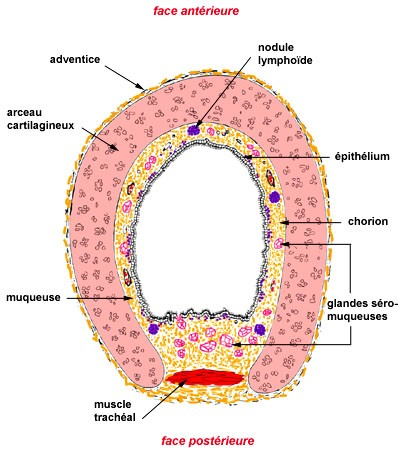
\includegraphics[scale=0.4]{gfx/Trach_esch_mas.jpg}
        \centering \caption{Schémas trachée}
        \label{Trachéeschémas}
    \end{minipage}\hfill
    \begin{minipage}[b]{0.7\linewidth}
        \centering 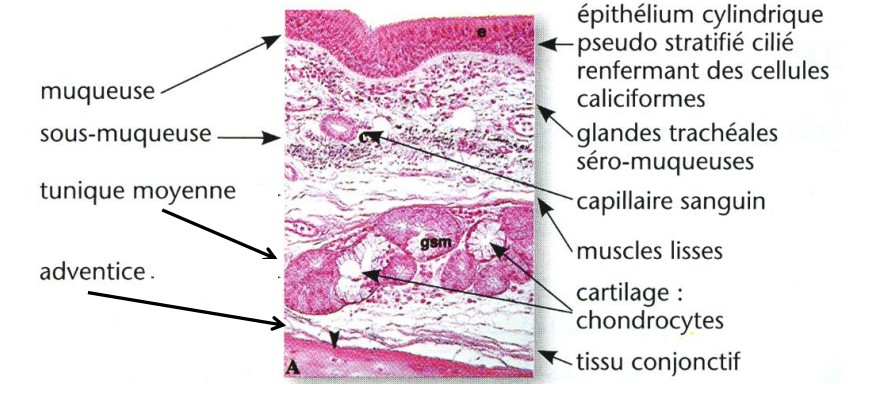
\includegraphics[scale=0.4]{gfx/Trach_ecoupe.jpg}
        \centering \caption{Coupe trachée}
        \label{Trachéecoupe}
    \end{minipage}
\end{figure}

La structure et la fonction de la trachée sont en relation étroite. De forme cylindrique elle assure le passage de l'air durant tout le cycle de la respiration, elle présente aussi, en relation avec son appareil mucociliaire, une fonction de drainage permettant l'élimination des particules inhalées vers le pharynx. (Figure \ref{Trachéeschémas} et Figure \ref{Trachéecoupe})

%------------------------------------------------

% \subsection{Subsection Title}

% Content
 % Chapter 1
% Chapter X

\chapter{Poumon} % Chapter title


\label{ch:01-02} % For referencing the chapter elsewhere, use \autoref{ch:name} 

%----------------------------------------------------------------------------------------

% \section{}

A la suite de la trachée on à l’organe central de la respiration, le poumon qui est situé dans la cage thoracique au-dessus du diaphragme. Une double membrane séreuse, la plèvre pariétale, située contre la paroi thoracique et la plèvre viscérale maintien le poumon contre la paroi thoracique. \\
\\
Hors pathologies, l’Homme possède deux poumons séparés l’un de l’autre par le médiastin. Le poumon dit droit est divisé en trois lobes et le gauche en deux, ceci étant dû à la place occupée par le cœur. Chacun de ces lobes est relié à la trachée via une bronche souche qui se divise en bronches plus petites, puis en bronchioles à l’extrémité desquelles on retrouve les alvéoles regroupées par grappe, lieux principal des échanges gazeux entre l'air baignant les alvéoles et le sang des capillaires. (Figure \ref{poumon})

\begin{center}
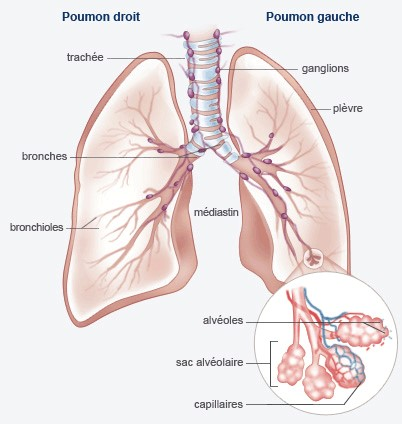
\includegraphics[scale=0.7]{gfx/poumon.jpg} 
\captionof{figure}{Poumon}
       \label{poumon}
\end{center}

		\section{Bronche et Bronchioles}
Les bronches primaires (ou souches) se divisent en bronches lobaires puis en bronches segmentaires pour finir par les bronchioles. D’architecture semblable à la trachée, les bronches primaires présentent un épithélium de type respiratoire identique à celui de la trachée mais aussi quelques différences: une discontinuité des anneaux cartilagineux, elles présentent également un réseau de fibres élastiques plus important dans le chorion qui fait office de séparation avec la sous muqueuse qui contient moins de structures glandulaires.\\
\\
Les bronchioles sont très fines (0.5 à 1mm de diamètre) divisées en trois types chacun étant progressivement de plus en plus petit : les bronchioles lobaires, les bronchioles terminales et les bronchioles respiratoires. Il n’y a pas d’échange d’air dans les bronchioles lobaire et terminales par contre on a un échange au niveau des bronchioles respiratoire. La fonction primaire des bronchioles est de conduire l’air des bronches aux alvéoles et de contrôler le débit d’air distribué dans le poumon par constriction ou dilatation. \\
\\
La structure des bronchioles est sensiblement différente des celles des bronches. Alors que les bronches sont entourées d’un anneau de cartilage qui permet de les maintenir ouvert, les bronchioles sont-elles entourées d’un mur de muscle lisse permettant de dilater et de contracter les voies respiratoires contrôlant ainsi la livraison d’air aux alvéoles. Leur muqueuse est formée d’un épithélium simple cylindrique dépourvu de cellules caliciformes et pauvre en cellules ciliées. Le chorion est réduit à une fine lame élastique et la sous muqueuse qui se confond avec l’adventice ne contient pas de glandes. (Figure\ref{bronche})

\begin{center}
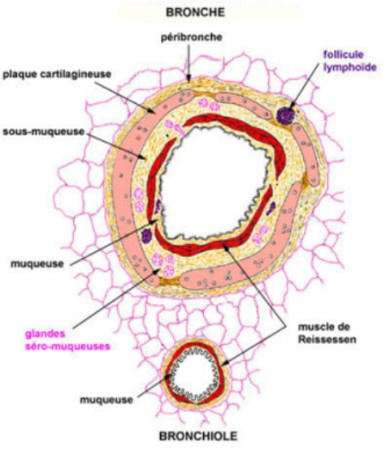
\includegraphics[scale=1.6]{gfx/bronche.jpg} 
\captionof{figure}{Bronche}
       \label{bronche}
\end{center}


		\section{Alvéoles}
A l’aboutissement de l’arbre bronchique on retrouve les alvéoles regroupées en acinus pulmonaire. Un acinus est constitué des 5 à 6 alvéoles entourées d’un réseau de capillaire sanguin fixé et intiment lié à la fonction des alvéoles.\\
\\
L’épithélium alvéolaire est constitué de pneumocytes de deux types différents type I (membraneux) et type II (granuleux). La barrière alvéolo-capillaire au travers de laquelle est assuré la fonction d’échanges gazeux est formée des Pneumocytes de type I des alvéoles et des cellules endothéliales des capillaires. \\
\\
Alors que la proportion en Pneumocytes I et II est sensiblement identique, les Pneumocytes de type I, du fait de leurs structures fines (0,1 à {0,2}{\micro\metre} d'épaisseur) et étalées, couvrent 95\% de la surface alvéolaire. Ceci a pour conséquence de conférer à l’épithélium alvéolaire une caractéristique souple très étendu qui favorise les échanges gazeux, mais aussi très fragile qui le rend vulnérable aux attaques microbiennes et aux polluants.\\
\\
Les pneumocytes de type II sont de forme cubique et présente une microvillosité au niveau de leurs pôle apical. Leurs aspect granuleux est dû à leur cytoplasme riche en organites dont un spécifique, les corps lamellaires qui sécrètent le surfactant pulmonaire, de plus ils présentent un réticulum endoplasmique et un appareil de Golgi surdéveloppés signe d’un métabolisme très actif. \\
Le surfactant sécrété (et aussi recyclé), par les corps lamellaires des pneumocytes de type II, a pour fonction de fluidifier le mucus et de facilite les échanges gazeux, de diminuer la tension de surface des alvéoles afin qu'elles ne s'effondrent pas sur elles-mêmes pendant la respiration et à la conservation de l'élasticité des poumons. (Figure \ref{alveol})


\begin{center}
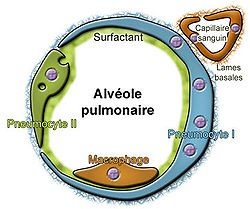
\includegraphics[scale=0.7]{gfx/alveole.jpg} 
\captionof{figure}{Alvéole}
       \label{alveol}
\end{center}

		\section{Pathologies}
Les maladies pulmonaires ont essentiellement des causes infectieuses (bactéries, virus ou champignons pathogènes). Le plus fréquent étant le pneumocoque (Streptococcus pneumoniae) qui est aussi l’un des plus dangereux. \\
Parmi les pathologies pulmonaires fréquentes on trouve l’asthme, les bronchopneumopathies chroniques obstructives (BCPO) caractérisé par un rétrécissement irréversible des bronches, cancers et la mucoviscidose maladie génétique caractérisé par une production importante d’un mucus épais qui entraîne d’important troubles respiratoires. On peut en citer pleins d’autre mais c’est sur cette dernière pathologie que notre étude se concentre.




%------------------------------------------------

% \subsection{Subsection Title}

% Content % Chapter 2


% \cleardoublepage % Empty page before the start of the next part

%------------------------------------------------

\ctparttext{} % Text on the Part 2 page describing the content in Part 2
% Soulever dans ce § les principales questions soulevées dans cette partie

\part{La Mucoviscidose} % Second part of the thesis

% Chapter X

\chapter{Généralité} % Chapter title


\label{ch:02-01} % For referencing the chapter elsewhere, use \autoref{ch:name} 

%----------------------------------------------------------------------------------------

% \section{}

La mucoviscidose est une maladie à transmission autosomique et récessive multiviscérale, autrement dit, c’est une maladie qui peut toucher de nombreux organes et seul les personnes ayant hérité de deux mutations, provenant l’un du père et l’autre de leur mère, sont atteintes. Elle touche essentiellement les personnes d’origine caucasienne et est très rarement retrouvé en Asie et en Afrique. La mucoviscidose est causé par des mutations dans un gène identifié en 1989 (Riordan et al. 1989)\cite{riordan_identification_1989} et localisé sur le bras long (appelé q) du chromosome 7 à la position 31.2 (7q31.2). Ce gène appelé CFTR (Cystic fibrosis transmembrane conductance regulator) code pour une glycoprotéine membranaire de même nom retrouvée au pôle apical de la majorité des cellules épithéliale. 
C’est en 1938 à la suite d’autopsie d’enfants souffrant de malnutrition que pour la première fois la distinction fut établie entre la maladie cœliaque et la mucoviscidose défini à l’époque par le terme de « fibrose cystique du pancréas ». Elle fut décrite comme une maladie caractérisée par une mauvaise absorption des graisses et protéines, une stéatorrhée (quantité élevée de lipides dans les selles), un retard de croissance et des infections pulmonaires (ANDERSEN DH 1938)\cite{andersen_dh_cystic_1938}. Ce n’est qu’en 1943 qu’elle fut renommé « mucoviscidose » afin de rendre compte de l’état visqueux du mucus généralisé à plusieurs organes autre que le pancréas (Farber 1943)\cite{farber_pancreatic_1943}. En 1948 lors de la vague de chaleur à New York un jeune pédiatre, Paul di Sant'Agnese, constata que beaucoup de nourrissons atteint de mucoviscidose présentaient une prostration due à la chaleur. Il émit l’hypothèse d’un problème de sudation et démontra un excès de sodium et de chlorure cinq fois plus important dans la sueur des patients atteints de mucoviscidose, qui persistait même après la vague de chaleur(Di Sant’agnese et al. 1953)\cite{di_santagnese_abnormal_1953}. C’est grâce à cette découverte que sera mis au point un peu plus tard le test de la sueur toujours utilisé de nos jours afin de diagnostiquer les patients (Gibson and Cooke 1959)\cite{gibson_test_1959}.
Selon le registre français de la mucoviscidose en 2014 on comptait un peu plus de 6000 patients recensés. Ce nombre, en constante progression depuis le début du recensement en 1992, compte pour la deuxième fois consécutive, même si la population reste jeune avec un âge moyen d’environ 20 ans, plus d’adultes que d’enfants. (Figure \ref{patient} et Figure \ref{evolutionpatient})
\begin{center}
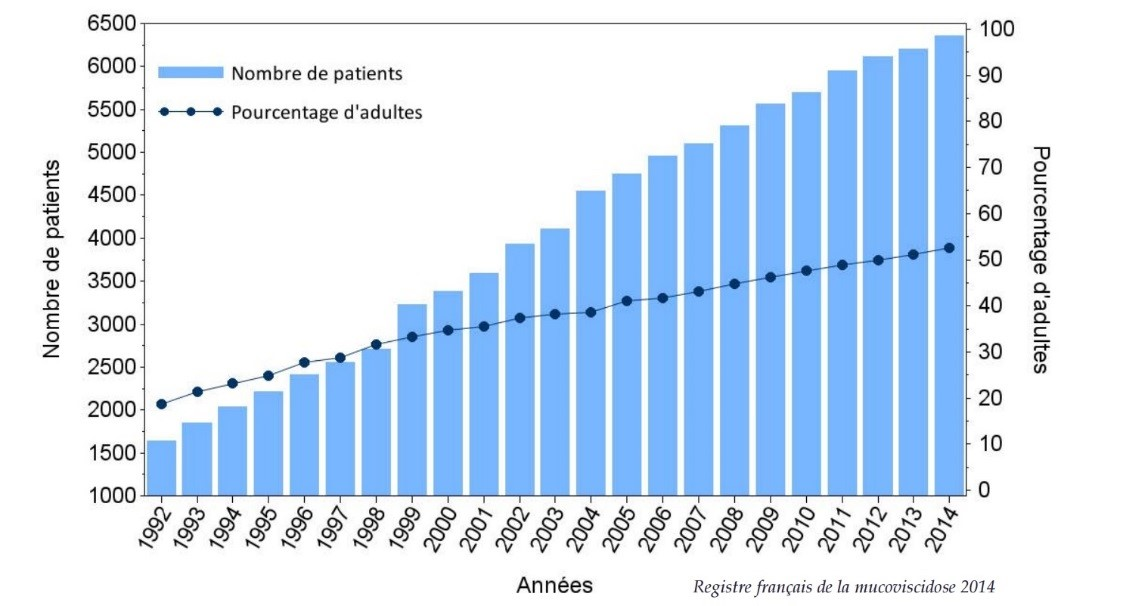
\includegraphics[scale=1]{gfx/patient.jpg} 
\captionsetup{type=figure}
\captionof{figure}{Nombre de patients vus dans l'année et pourcentage d'adultes (registre français de la mucoviscidose)}
       \label{patient}
\end{center}
\begin{center}
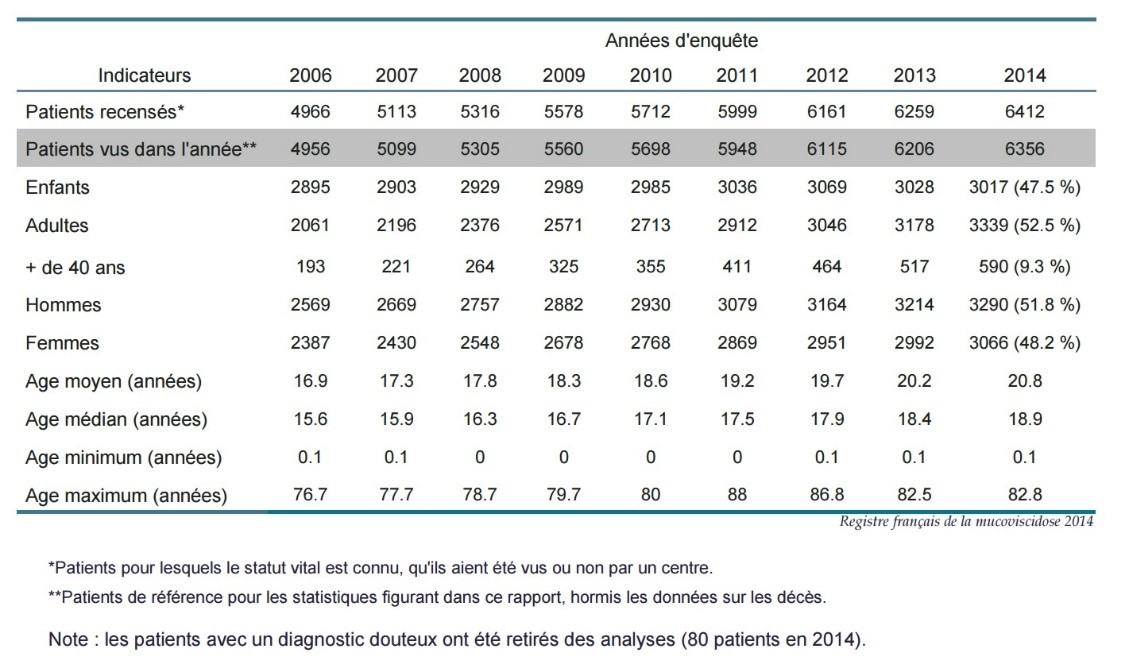
\includegraphics[scale=1]{gfx/evolutionpatient.jpg} 
\captionsetup{type=figure}
\captionof{figure}{Evolution annuelle des principaux indicateurs (registre français de la mucoviscidose)}
       \label{evolutionpatient}
\end{center}
	
%------------------------------------------------

% \subsection{Subsection Title}

% Content % Chapter 1
% Chapter X

\chapter{Données clinique}

\label{ch:02-02} % For referencing the chapter elsewhere, use \autoref{ch:name} 
%----------------------------------------------------------------------------------------

% \section{}

La fonction de CFTR est de réguler le transport des ions et les mouvements d’eau au travers de la barrière épithéliale des cellules qui produisent du mucus, de la sueur ou de la salive. Sans altération CFTR fonctionne comme un canal à travers la membrane et transporte les ions chlorure négativement chargé en dehors de la cellule afin d’aider au contrôle des mouvements d’eau dans les tissus, élément nécessaire pour la production d’un fin mucus qui va protéger les voies aériennes, le système digestif et reproducteur, ainsi que d’autre organes et tissues.

Parmi les organes atteints par la mucoviscidose, les atteintes pulmonaires sont les plus graves car elles se révèlent fatal dans la plupart des cas. Succinctement, le gène CFTR défectueux est à l’origine d’une absorption de l’eau contenue dans le mucus qui protège les voies respiratoires. Cette couche fine devenue visqueuse empêche les cellules ciliaires de battre et donc les mécanismes d’évacuation du mucus de fonctionner correctement. Ainsi, l’ensemble des particules inhalées reste retenues à la surface des voies aériennes et des bactéries trouvent ainsi un environnement favorable à leurs proliférations.

Les atteintes pancréatiques, elles, vont avoir pour conséquence une difficulté d’assimilation des nutriments, le pancréas très abîmé de naissance et encombré par un épaississement du mucus empêche la bonne libération des enzymes essentielles à une bonne digestion. Le foie et le système digestif atteint aussi, peuvent présenter une cirrhose biliaire pour le premier et une constipation et obstruction intestinale pour le second. Un retard de la puberté et une infertilité peut aussi toucher certains patients (Figure \ref{organe}).

On peut observer une large diversité d’expression clinique d’un patient à l’autre, que ce soit pour l’âge d’apparition des premiers symptômes ou la sévérité de l’évolution de la maladie mais un déclin des fonctions pulmonaire caractérisé par une infection progressive des voies respiratoires ainsi qu’une inflammation reste la cause principale de mortalité et morbidité.

\begin{center}
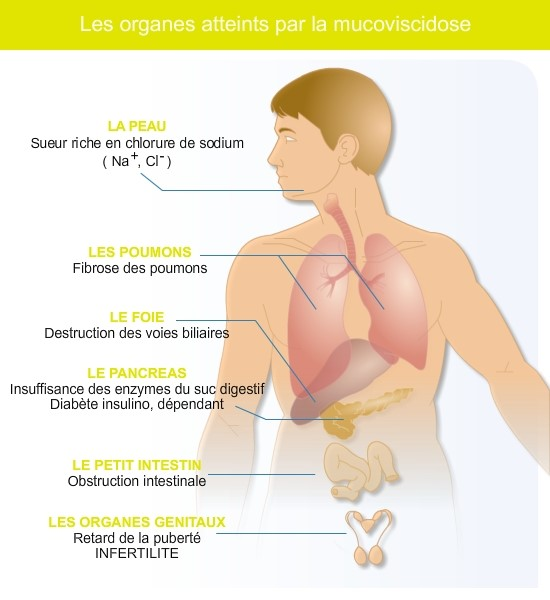
\includegraphics[scale=0.5]{gfx/organes.jpg} 
\captionsetup{type=figure}
\captionof{figure}{organes atteints par la Mucoviscidose}
       \label{organe}
\end{center}
 % Chapter 2
% Chapter X

\chapter{Approches thérapeutiques fondamentales} % Chapter title


\label{ch:02-03} % For referencing the chapter elsewhere, use \autoref{ch:name} 

%----------------------------------------------------------------------------------------

% \section{}
Depuis la découverte de CFTR de nombreux progrès en termes de soin médicaux ont été fait, mais bien que l’espérance de vie soit d’environ une cinquantaine d’année en moyenne pour les patients, la mucoviscidose reste une maladie incurable, mais la question est, pourquoi ?
La première des raisons réside dans le fait que le gène, cause première de la maladie, n’a été découvert que très récemment. Depuis cette découverte de nombreux progrès en termes de soin médicaux ont été fait, d’ailleurs, Il existe deux approches thérapeutiques fondamentales. La première consiste à cibler les problèmes pulmonaires en s’attaquant aux infections microbiennes ou tenter de modifier la couche de mucus. La seconde consiste à cibler les causes premières de la maladie, c’est-à-dire refaire fonctionner la protéine CFTR défectueuse ou bien la remplacer par thérapie génique ou à l’aide d’autres moyens pharmacologiques. Les thérapies ciblant les causes premières sont le plus souhaitable à l’avenir pour le traitement de la mucoviscidose, mais de tels traitements sont difficiles à développer.
La première des approches thérapeutiques fondamentales consiste en des traitements multiples destinés à soulager les symptômes de la maladie, mais ils sont contraignants de par le fait qu’ils nécessitent un suivi quotidien. L’un des traitements essentiels de la mucoviscidose et aussi la plus contraignante est la kinésithérapie respiratoire qui permet de désencombrer les bronches, mais il faut l’effectuer plusieurs fois par jour pendant 1h environ. En complément sont prescrit au patient des antibiotiques, des anti-inflammatoires et des médicaments permettant de fluidifier le mucus afin de soulager les troubles respiratoires. Seulement ces traitements ne visent qu’à soigner les conséquences et non les causes de la maladie. C’est pourquoi actuellement la deuxième des approches thérapeutiques fondamentales est la plus investigué en recherchant un traitement curatif visant à identifier et à contrôler les actions des transporteurs comme CFTR causant la déshydratation du mucus qui est à l’origine de ces troubles. Comme décrit précédemment le dysfonctionnement de la protéine CFTR serait à l’origine de la maladie, il semble donc logique de penser qu’une correction de son activité soit la clé de la guérison pour les patients. C’est pourquoi de nombreux travaux ont été effectués afin de restaurer l’activité de CFTR directement ou indirectement et ce grâce à de nombreuses molécules ou par correction génétique de la mutation responsable. En effet la restauration de la sécrétion chlorure est l’enjeu majeur du développement de thérapeutiques pharmacologique de la mucoviscidose. A ce jour il est possible d’agir grâce à des composants pharmacologiques sur CFTR en ciblant son système de régulation ou directement sur le canal par l’intermédiaire d’activateurs ou de potentiateurs de CFTR directs ou indirects.


%------------------------------------------------

% \subsection{Subsection Title}

% Content % Chapter 3
% Chapter X

\chapter{CFTR} % Chapter title


\label{ch:02-03} % For referencing the chapter elsewhere, use \autoref{ch:name} 

%----------------------------------------------------------------------------------------

% \section{}
\section{Structure}
CFTR (ABCC7) est une glycoprotéine membranaire de taille et de poids moléculaire important  (1480 acides aminés et 170kDa). Elle appartient à la superfamille des transporteurs ABC (ATP Binding Cassette) et plus précisément à la sous famille ABCC.
La famille des transporteurs ABC est une famille extrêmement vaste de protéines, on les retrouve dans l’ensemble du vivant aussi bien eucaryote que procaryotes (Hyde et al. 1990)\cite{hyde_structural_1990}. Leurs particularité est qu’elles sont capable de lier ainsi que d’hydrolyser l’ATP. Elles utilisent l’énergie issu de cette hydrolyse pour effectuer des échanges unidirectionnels d’éléments divers (ions, substrats, macromolécules…) au travers des membranes cellulaire (Higgins 1992)\cite{higgins_abc_1992}. Les transporteurs ABC sont constitué de quatre domaines : deux domaines NBD (nucleotide binding domains) cytoplasmiques qui ont la capacité de lier les nucléotides et deux domaines transmembranaires TMD (transmembrane domains). Sauf quelques exceptions les TMD sont composés de 6 segments transmembranaires dont la nature dépend de l’élément transporté. Les NBD possèdent trois motifs très conservées, les motifs Walker A et B de fixation de l’ATP et un motif dit « signature » LSGGQ, spécifique des transporteurs ABC, et situé entre le motif de Walker A et B (Walker et al. 1982)\cite{walker_distantly_1982}. Le passage des éléments à travers la membrane cellulaire se fait généralement grâce à l’énergie résultant de l’hydrolyse de l’ATP, sauf pour certains transporteurs comme CFTR où la présence d’autres domaines influence le transfert (Biemans-Oldehinkel, Doeven, and Poolman 2006)\cite{biemans-oldehinkel_abc_2006}.
Très peu de structures tridimensionnelles des membres de la superfamille des transporteurs ABC sont disponibles à ce jour, mais l’analyse de la séquence de CFTR nous indique qu’il est constitué de deux domaines TMD 1 et 2 de six segments transmembranaires et de trois domaines intracellulaires : deux domaines NBD 1 et 2 et un domaine régulateur R reliant le NBD 1 au TMD2 et possédant de nombreux sites de phosphorylation (Devidas and Guggino 1997)\cite{devidas_cftr:_1997}. Le domaine régulateur R est codé par un exon unique, le 13ème exon, et n’est retrouvé que chez CFTR. Afin de permettre l’ouverture du canal par le MgATP sa phosphorylation préalable par les protéines kinases A et C (PKA, PKC) est nécessaire. On retrouve aussi au niveau de la 4ème boucle extracellulaire reliant les segments transmembranaires TM7 et TM8 deux sites de N-glycosylation au niveau des asparagines 894 et 900 (N894 et N900). La grande majorité de la protéine (environ 80\%), est cytoplasmique dont ses domaines N et C terminaux, le reste étant soit transmembranaire (16\%) soit extracellulaire (4\%). (Akabas, Cheung, and Guinamard 1997; Rosenberg et al. 2004)\cite{akabas_probing_1997}\cite{rosenberg_purification_2004} (Figure \ref{cftr}).
\begin{center}
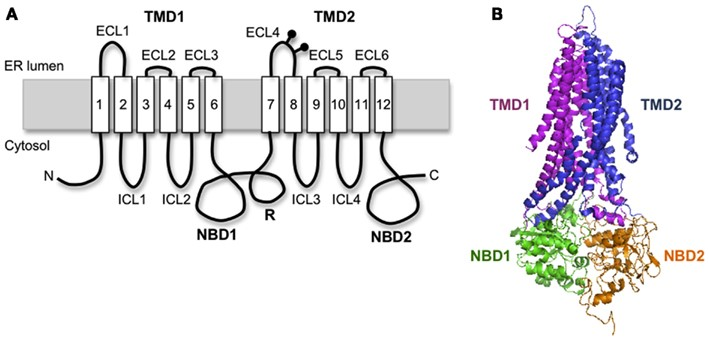
\includegraphics[scale=2]{gfx/CFTR.jpg} 
\captionof{figure}{Structure CFTR}
       \label{cftr}
\end{center}

		\section{Fonction}
Le rôle de la protéine CFTR est toujours sujet à spéculations, mais il est maintenant admis que CFTR est une protéine multifonctionnelle. Une de ces fonctions principale est d’être un canal chlorure indépendant du voltage et du temps, mais dépendant de l’AMPc (régulation via PKA et PKC par phosphorylation), utilisant l’hydrolyse de l’ATP comme énergie et ayant une faible conductance (Anderson, Berger, et al. 1991; Anderson, Gregory, et al. 1991)\cite{anderson_nucleoside_1991}\cite{anderson_demonstration_1991}. CFTR forme un canal anionique permettant la diffusion passive des ions chlorure, le mécanisme de sélectivité de charge est lié aux segments transmembranaires TM1 et TM6. (Dawson, Smith, and Mansoura 1999; Linsdell 2006)\cite{dawson_cftr:_1999}\cite{linsdell_mechanism_2006}. La séquence de sélectivité du canal CFTR est : Br- (Bromure)>Cl- (Chlorure)>I- (Iodure)>F-(Fluorure). Cette perméabilité du Cl- plus importante que celle de l’I- différencie CFTR des autres canaux chlorure pour qui cette séquence est inversée(Sheppard and Welsh 1999)\cite{sheppard_structure_1999}. Possédant une sélectivité plus grande pour les anions plutôt que pour les cations monovalents, CFTR semble aussi perméable au tripeptide glutathion (GSH) qui est l’antioxydant le plus abondamment retrouvé dans les poumons (Kogan et al. 2003)\cite{kogan_cftr_2003}.
CFTR est aussi une protéine régulatrice de courant chlorure, elle possède donc aussi des propriétés de régulation de la conductance membranaire. Elle a été montrée comme étant un acteur majeur de la régulation du canal ORCC (Outwardly Rectifying Chloride Channel) de par sa présence fonctionnelle indispensable à l'activation du canal ORCC par les PKA(Devidas and Guggino 1997)\cite{devidas_cftr:_1997}. CFTR est aussi régulatrice d’autres protéines comme le canal sodique ENaC (Epithelial Na+ Channel), elle le régule négativement(Devidas and Guggino 1997)\cite{devidas_cftr:_1997}. Son absence entraine une hyper-absorption de Na+ ce qui a pour conséquence la déshydratation du mucus (Letz and Korbmacher 1997)\cite{letz_camp_1997}. Pour l’inhibition des canaux potassiques ROMK (Renal Outer Medullary Potassium channel) par l’ATP cytosolique, CFTR est nécessaire (Ruknudin et al. 1998)\cite{ruknudin_novel_1998}. Enfin une régulation positive des aquaporines par CFTR participe à l’hydratation du mucus (Schwiebert et al. 1999; Schreiber et al. 2000) \cite{schwiebert_cftr_1999}\cite{schreiber_aquaporin_2000}
En conclusion la fonction de CFTR est de réguler le transport des ions et les mouvements d’eau au travers de la barrière épithéliale des cellules qui produisent du mucus, de la sueur ou de la salive. Sans altération CFTR fonctionne comme un canal à travers la membrane et transporte les ions chlorure négativement chargé en dehors de la cellule afin d’aider au contrôle des mouvements d’eau dans les tissus, élément nécessaire pour la production d’un fin mucus qui va protéger les voies aériennes, le système digestif et reproducteur, ainsi que d’autre organes et tissues. 

		\section{Mutation CFTR}
Jusqu’à présent plus de 1900 mutations ont été identifié. Dans l’ensemble des mutations recensées, les plus communes sont les mutations faux-sens (48.7\%), suivi par des modifications du cadre de lecture causé par une petite insertion ou délétion (19.5\%), puis des mutations altérant des codons essentiels pour l’épissage (15.7\%) et enfin des mutations non-sens (12.9\%). En fonction du dysfonctionnement moléculaire observé sur CFTR ces mutations ont été réparties dans différentes catégories, on dénombre six classes (Kerem 2006)\cite{kerem_mutation_2006}. Alors que les trois dernières classes sont associées à un phénotype mucoviscidosique modéré, les trois premières sont beaucoup plus sévères (Figure \ref{mutation}):
\begin{itemize}
\item Mutations de classe I conduisent à un défaut de production de la protéine CFTR qui est complétement absente, ce sont les deuxièmes mutations les plus communes.
\item Mutations de classe II conduisent à un défaut de maturation de CFTR, ce qui a pour conséquence d’affecter l’adressage de la protéine dans le réticulum endoplasmique et l’appareil de golgi. Ceci est dû à une mauvaise glycosylation et repliement de la protéine ne formant pas une structure tertiaire appropriée et qui finit donc par être ciblé par la dégradation au lieu d’être envoyée à la membrane apicale. Ce sont les mutations les plus communes on y retrouve la mutation $\Delta508$F qui représente 70\% des mutations observé chez les patients atteint de mucoviscidose. 
\item Mutations de classe III et IV, la protéine CFTR est normalement traduite et normalement adressé à la membrane apicale, mais il manque une complète activité de son canal ionique. Dans le cas des mutations de classe III on a un défaut de régulation de CFTR dû à une diminution de la probabilité d’ouverture du canal. Pour les mutations de classe IV on a une altération de la conduction du canal, les mutations peuvent induire des modifications de sa sélectivité ainsi qu’une diminution du flux ionique. 
\item Mutations de classe V résulte en une altération de stabilité de l’ARN messager conduisant à un nombre diminué de copie de CFTR et donc à un trafique appauvrie à la membrane plasmique. 
\item Mutations de classe VI sont à l’origine d’une altération de stabilité de la protéine mature, on a une accélération du turnover de la protéine CFTR à la surface de la cellule et donc à une diminution de sa quantité.
\end{itemize}

\begin{center}
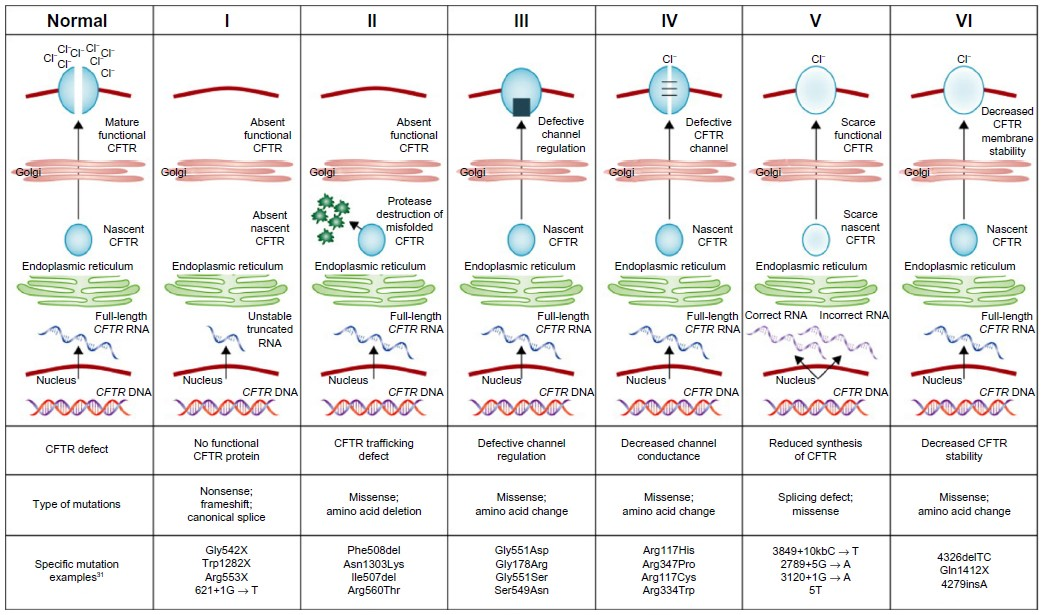
\includegraphics[scale=0.4]{gfx/mutation.jpg} 
\captionof{figure}{Classes de mutation de CFTR}
       \label{mutation}
\end{center}
 
Ces mutations ont de multiples conséquences principalement un défaut de transport d’ion et de mouvement d’eau à l’intérieur et l’extérieur de la cellule et qui a pour conséquence une production d’un mucus épais par les organes à tissus épithéliaux sécréteurs. Ce mucus va notamment avoir pour effet d’obstruer les voies respiratoires et les glandes, menant à des signes et symptômes caractéristiques de la mucoviscidose notamment une inflammation chronique qui reste la cause principale de mortalité et morbidité

%------------------------------------------------

% \subsection{Subsection Title}

% Content % Chapter 4
% Chapter X

\chapter{Inflammation dans la mucoviscidose} % Chapter title


\label{ch:02-04} % For referencing the chapter elsewhere, use \autoref{ch:name} 

%----------------------------------------------------------------------------------------

% \section{}

\section{Inflammation généralité}
Nous vivons dans un monde inondé d’agresseurs trop petit pour être détectés à l’œil nu, et aucun vertébré ne pourrait résister longtemps à leur attaque s’il n’était protégé. Nous survivons parce que nous avons acquis au cours de l’évolution divers mécanismes de défenses très efficaces contre ces attaques permanente et il importe de garder à l’esprit que bien qu’efficace ils sont loin d’être parfait. 
Un vertébré se défend contre une infection à l’instar d’un chevalier qui défendait les cités médiévales. Les « remparts et les fossés » rende l’invasion difficile, les « sentinelles » interpelles tout ce qui erre dans les environ et font appel aux « patrouilles » si un inconnu ne peut prouver son innocence :
\begin{itemize}
\item Les remparts et fossés : la peau, couche externe du corps des vertébré, est la première barrière que doivent franchir les microbes. Les muqueuses des tractus respiratoire, digestif et urogénital font également partie de l’enceinte protectrice.
\item Les sentinelles : Appartenant au système immunitaire certaines de ces cellules sont particulièrement agressives et tuent (par phagocytose) tous éléments reconnus comme étrangers, ou les virus afin qu’ils soient reconnus et éliminés par les patrouilles. Les cellules sentinelles (ou résidantes des tissus) comprend les phagocytes mononucléés résidents (cellules dendritiques et macrophages) ainsi que les mastocytes. Si cette première ligne de défense des sentinelles était franchie, l’organisme réagirait en organisant une contre-attaque cellulaire capable de tuer l’élément étranger. Ce moyen de défense entre en action très rapidement après le début de l’infection. Elles sont activées en contact avec les éléments étrangers, en réponse elles vont libérer des médiateurs de l’inflammation notamment des cytokines pro-inflammatoires et de l’histamine, un vasodilatateur qui va favoriser le recrutement des « patrouilles » dans les tissus.
\item Les patrouilles : Les cellules qui patrouillent via le sang dans l’ensemble de l’organisme sont les lymphocytes T et B, les cellules NK, les monocytes qui vont maturer en macrophages en gagnant le tissu où ils seront qualifiés de résident, et la famille des granulocytes dont l’activité s’exerce au niveau des tissus et qui comprend les polynucléaires basophiles, éosinophiles et neutrophiles. Ces cellules comptent parmi les leucocytes les plus nombreux dans la circulation périphérique. Ils ont un noyau multilobé et de nombreuses granules dans leur cytoplasme, entre les divers types de granulocytes d’importantes différences fonctionnelles existent. 
\end{itemize}
Patrouilles et sentinelles forment l’inflammation et constitue l’un des mécanismes les plus importants des défenses de l’organisme. Il existe de multiples causes à l’origine de l'inflammation, comme les agressions de types physiques (traumatisme, chaleur/ froid, radiations) ou chimiques (agents caustiques, toxines, venins).il y a aussi l’infection par des micro-organismes comme les bactéries, virus, parasites et champignons ou une agression dys-immunitaire (anomalie de la réponse immunitaire, allergies …) qui sont capable de déclencher une inflammation. Dans tous les cas l’agent pathogène peut être soit endogène ou exogène, plusieurs causes peuvent être associées dans le déclenchement de l’inflammation et pour un même agent pathogène on peut avoir des réactions inflammatoires différentes selon l’hôte et l’état de ses défenses immunitaire. (Figure \ref{inflammation})
\begin{center}
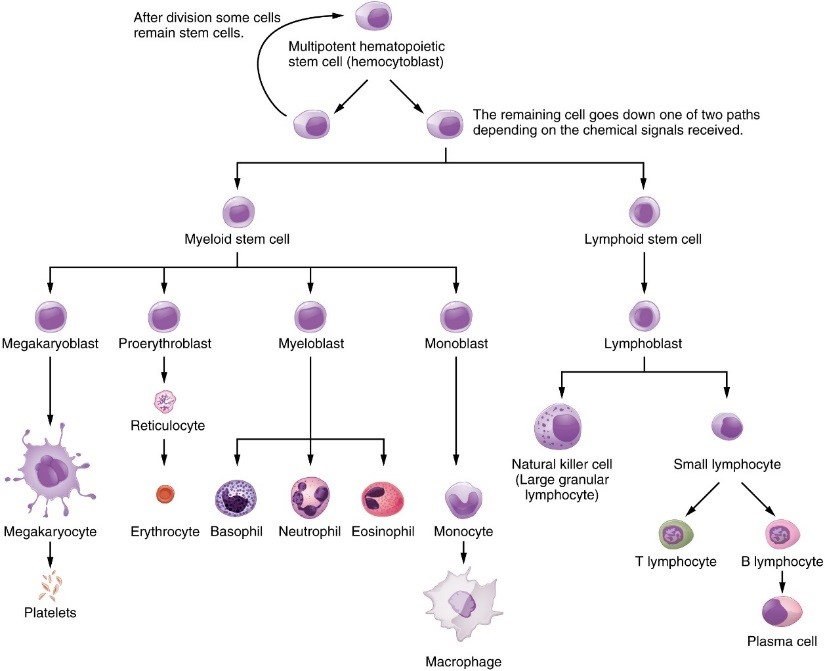
\includegraphics[scale=1]{gfx/inflammation.jpg} 
\captionof{figure}{Cellules de l'inflammation}
       \label{inflammation}
\end{center}

La réaction inflammatoire ou inflammation est définie comme la réponse locale à toutes sortes d’agression de tissus vascularisé et vivant. Habituellement bénéfique pour l’organisme, ce processus a pour but de réparer les lésions et d’éliminer l’agent pathogène, mais peut conduire dans certain cas à une inflammation néfaste pour l’organisme en raison de l’agressivité ou de la persistance de cet agent. D’autres causes, comme des anomalies dans la régulation du processus inflammatoire ou lorsque la quantité ou la qualité des éléments intervenant dans l’inflammation sont altérés peuvent aussi conduire à une inflammation néfaste. Ce qui est le cas dans la mucoviscidose qui est caractérisée par des atteintes pulmonaires progressives graves qui sont la cause principale de mortalité et morbidité chez les patients.

		\section{Cas de la mucoviscidose}
Au cours de ces 30 dernières années de nombreuse recherche ont été effectué concernant l’origine de cette réponse inflammatoire qui commence très tôt, qui persiste, qui deviens excessive à la suite d’une infection et qui se révèle le plus souvent inefficace dans la mucoviscidose (Nixon et al. 2002; Khan et al. 1995; Balough et al. 1995; Chen and Nuñez 2010; Pillarisetti et al. 2011)\cite{nixon_early_2002}\cite{khan_early_1995}\cite{balough_relationship_1995}\cite{chen_sterile_2010}\cite{pillarisetti_infection_2011}. La libération d’élastase et d’autre protéinase par les neutrophiles est considérée comme l’élément clé contribuant aux dommages pulmonaire associé à la réponse inflammatoire (Armstrong et al. 1995)\cite{armstrong_lower_1995}. Chez les patients atteints de mucoviscidose l’activité de l’élastase et des autres protéines est très élevée comparé à ceux des personnes non atteints (Downey, Bell, and Elborn 2009)\cite{downey_neutrophils_2009}. On constate aussi des changements structurels aux niveaux des voies aériennes et un encombrement des bronchioles dû à l’épais mucus produit par les glandes sécrétrices hypertrophiées(Hays and Fahy 2006)\cite{hays_characterizing_2006}. 
Parmi les pathogènes qui colonise les voies aérienne des patients atteint de mucoviscidose les plus fréquemment retrouvés sont Pseudomonas Aeruginosa, Staphylococcus Aureus et Haemophilus Influenzae (Saiman 2004)\cite{saiman_microbiology_2004}. Souvent la réponse des patients à l’infection est excessive. Une bronchectasie finie par se développer à cause d’une obstruction des voies respiratoire et des infections bactériennes constantes liées à une réponse inflammatoire exacerbée. Depuis peu le précepte considérant que l’infection initie l’inflammation est remis en question. La mutation CFTR étant elle-même capable d’induire directement l’inflammation en absence d’infection (Rao and Grigg 2006)\cite{rao_new_2006}. Tout ceci montre l’importance de l’inflammation dans la mucoviscidose. 

			\subsection{Mécanismes cellulaire des réactions inflammatoires }
			 \subsubsection{Macrophages}
Dans la mucoviscidose a été observé un défaut dans plusieurs fonctions des macrophages (Hubeau, Puchelle, and Gaillard 2001)\cite{hubeau_distinct_2001}. Ils présentent une diminution de leurs capacités de clearance des cellules apoptotique(Vandivier, Fadok, Hoffmann, et al. 2002; Vandivier, Fadok, Ogden, et al. 2002)\cite{vandivier_elastase-mediated_2002}\cite{vandivier_impaired_2002}, de la production de cytokines(Bonfield et al. 1995)\cite{bonfield_normal_1995} et de la phagocytose(Knight et al. 1997; Di et al. 2006)\cite{knight_defective_1997}\cite{di_cftr_2006}. Il semble aussi qu’il y a une dérégulation dans le recrutement de macrophages et de leurs fonctions bien avant leurs stimulations par l’infection(Starner et al. 2003)\cite{starner_ccl20_2003}. 

			\subsubsection{Neutrophiles }
Les fonctions des neutrophiles sont la défense de l’hôte, la phagocytose et la destruction de pathogènes invasifs(Hampton, Kettle, and Winterbourn 1998)\cite{hampton_inside_1998}. En réponse à une infection les neutrophiles génèrent des espèces réactives de l’oxygène (ROS) via la NADPH oxydase et secrète des protéines granulaires anti microbiennes comprenant entre autre l’élastase, la collagénase, les cathepsines et la myeloperoxidase afin de protéger l’organisme. De l’ADN peut être libéré par les neutrophiles pour former des NETS (neutrophil extracellular traps) qui vont piéger les bactéries afin de les éliminer(Brinkmann et al. 2004; Brinkmann and Zychlinsky 2007)\cite{brinkmann_neutrophil_2004}\cite{brinkmann_beneficial_2007}. Si cette réponse est non contrôlée, il peut en résulter des dommages aux tissues excessifs graves et qui représentent la majorité des dommages pulmonaire observées chez les patients atteint de mucoviscidose. Sous hypoxique, condition caractéristique d’un mucus mucoviscidosique, les neutrophiles vivent plus longtemps, augmentant ainsi leurs potentiels d’endommagement du poumon(Walmsley et al. 2005)\cite{walmsley_hypoxia-induced_2005}. Chez des enfants et fœtus atteint de mucoviscidose on dénombre une quantité important de neutrophiles au niveau des voies respiratoires qui augmente au fur et à mesure que la maladie progresse(Rosenfeld et al. 2001; Muhlebach and Noah 2002)\cite{rosenfeld_early_2001}\cite{muhlebach_endotoxin_2002}. De plus il a été montre qu’il y a un défaut dans le contrôle de la réponse inflammatoire à la suite d’une stimulation qui est associé à une inhabilité à phagocyter et à débarrasser les poumons des bactéries(Armstrong et al. 1995)\cite{armstrong_lower_1995}. Un nombre certains d’études on montrés une multitude de différences entre les neutrophiles issus de patients atteint de mucoviscidose et ceux de patients sains notamment une augmentation de la production de ROS(Graff, Schram-Doumont, and Szpirer 1991)\cite{graff_defective_1991}, une augmentation de la dé-granulation(Koller, Urbanek, and Götz 1995)\cite{koller_increased_1995}, une augmentation dans l’activité protéolytique avec une augmentation de la libération d’élastase(Gaggar et al. 2007; Brockbank et al. 2005)\cite{gaggar_matrix_2007}\cite{brockbank_effect_2005} et de Métalloprotéinase matricielle (MMP)(Ratjen et al. 2002; Sagel, Kapsner, and Osberg 2005; Gaggar et al. 2007)\cite{ratjen_matrix_2002}\cite{sagel_induced_2005}\cite{gaggar_matrix_2007}, une augmentation de l’apoptose(Watt et al. 2005; Vandivier, Fadok, Ogden, et al. 2002)\cite{watt_neutrophil_2005}\cite{vandivier_impaired_2002}, une diminution dans l’activité antimicrobienne(Moraes et al. 2006) \cite{moraes_abnormalities_2006}et une dérégulation dans la production de cytokines(Corvol et al. 2003)\cite{corvol_distinct_2003}.

			\subsubsection{Epithélium}
L’épithélium pulmonaire participe activement à l’immunité innée et orchestre les réponses inflammatoires. L’interaction des pathogènes avec l’épithélium des voies aérienne est une étape indispensable à l’activation des mécanismes de défense impliquant les neutrophiles et les macrophages. La stimulation de l’épithélium par les pathogènes se fait via l’activation des toll-like récepteurs (TRL)(Machen 2006; Muir et al. 2004)\cite{machen_innate_2006}\cite{muir_toll-like_2004} par différents ligand (lipopeptides, peptidoglycane, acide lipotéichoïque, fragment CXCR1) et l’activation des voies de transcription AP-1 et NF-$\kappa$B (Moskwa et al. 2007)\cite{moskwa_novel_2007} résultant à la production de cytokine pro inflammatoire responsable du recrutement des leucocytes et monocytes(Zhang et al. 2005)\cite{zhang_human_2005}. 
En temps normal l’induction d’ARN messager de cytokine pro-inflammatoire comme entre autre IL-8, GRO-$\alpha$, MIP-3 diminue après une exposition chronique aux produits bactériens. Par contre la production de cytokine suite à une infection par Pseudomonas Aeruginosa ne baisse pas nécessairement chez les patients atteints de mucoviscidose suggérant une inflammation soutenue des voies aérienne(Nichols, Chmiel, and Berger 2008)\cite{nichols_chronic_2008}.
Plusieurs défauts ont été proposés à ce jour en relation avec la fonction épithéliale dans la réponse inné, notamment un défaut dans le contrôle de l’équilibre redox qui est sans aucun doute le plus marquant. En effet une diminution de la fonction CFTR a été montrée comme associée à une diminution du transport de la GSH dans la lumière des voies respiratoires(Gao et al. 1999; Velsor, van Heeckeren, and Day 2001)\cite{gao_abnormal_1999}\cite{velsor_antioxidant_2001}. Il a été montré aussi qu’un défaut de CFTR entraine un effet sur l’expression des gènes associé à la balance redox(Xu et al. 2006)\cite{xu_functional_2006} et présente une augmentation du stress oxydatif dans les voies respiratoires de jeunes patients atteint de mucoviscidose(Kettle et al. 2004)\cite{kettle_myeloperoxidase_2004}. De plus un défaut de l’activité oxydative des cellules de l’épithélium a été montré comme associé à un défaut dans l’activité bactéricide des cellules(Moskwa et al. 2007)\cite{moskwa_novel_2007}. Tout ceci porte à croire qu’un défaut dans le contrôle de l’équilibre redox semble être à l’origine des problèmes inflammatoires observés chez les patients atteints de mucoviscidose.


%------------------------------------------------

% \subsection{Subsection Title}

% Content % Chapter 4

\cleardoublepage % Empty page before the start of the next part


% %------------------------------------------------

\ctparttext{} % Text on the Part 3 page describing the content in Part 3

\part{Le stress oxydatif dans la mucoviscidose} % Third part of the thesis

% Chapter X

\chapter{Généralité} % Chapter title


\label{ch:03-01} % For referencing the chapter elsewhere, use \autoref{ch:name} 

%----------------------------------------------------------------------------------------

% \section{}

Lorsque la balance entre antioxydant et oxydant n’est plus capable de prévenir les altérations des fonctions physiologiques il se met en place ce que l’on définit d’état de stress oxydatif. 

Dans les voies respiratoires en particulier, ce que l’on appelle les ROS, terme générique qui regroupe nombre d’éléments et molécules très réactives, peuvent avoir des effets bénéfiques ou non en fonction de leurs concentrations. Tous organismes aérobies produisent des espèces réactives de l’oxygène (ROS) et de l’azote (RNS). Les ROS sont des espèces chimiques réactives contenant de l’oxygène radicalaire comme le radical superoxyde \textit{O}$_{2}$\up{-}, le radical hydroxyle (OH) et non radicalaire comme le peroxyde d’hydrogène (\textit{H}$_{2}$\textit{O}$_{2}$). Les ROS sont aussi bien produits de manière endogène qu’exogène. L’un des gros producteurs de ROS endogène est les complexes NADPH oxydase (NOX) présent dans les membranes cellulaires, la mitochondrie, les peroxysomes et le réticulum endoplasmique, il en existe 7 isoformes distinct. Polluants, tabac, radiation sont eux des producteurs exogènes. Les métaux tels que le fer, le cuivre, le chrome, le vanadium et le cobalt sont capables de faire un cycle redox dans lequel un seul électron peut être accepté ou donné par le métal. Cette action catalyse la production de radicaux et d'espèces réactives d'oxygène. La présence de ces métaux sous une forme non complexée peut augmenter considérablement le niveau de stress oxydatif. On pense que ces métaux induisent des réactions de Fenton et la réaction de Haber-Weiss, dans laquelle le radical hydroxyle est généré à partir du peroxyde d'hydrogène.
Les RNS sont une famille des molécules antimicrobiennes dérivées du monoxyde d'azote et du radical superoxyde produit respectivement via l’oxyde nitrique synthase (NOS) et NADPH oxydase.

La production de ROS est un processus physiologique nécessaire dans de nombreuses fonctions cellulaires. Plusieurs voies de signalisations sont régulées par les ROS parmi elles la voix des MAPK, JNK et de nombreuses autres. Une signalisation efficace et normale nécessite un déséquilibre court de la balance redox. Pourtant un stress oxydatif peut survenir lorsque qu’une augmentation de la production de ROS n’est pas finement régulée par les antioxydants et que celle-ci perdure dans le temps. 
Ainsi il a été montré qu’un excès de ROS peut favoriser la transcription de gènes pro-inflammatoire (Bartling and Drumm 2009)\cite{bartling_oxidative_2009} et parmi les dommages dû à un excès de ROS, l’oxydation peut causer des dommages irréversibles à de nombreuses cibles moléculaires notamment les lipides mais aussi l’ADN (Genestra 2007)\cite{genestra_oxyl_2007}.


%------------------------------------------------

% \subsection{Subsection Title}

% Content % Chapter 1
% Chapter X

\chapter{Dans la Mucoviscidose} % Chapter title


\label{ch:03-02} % For referencing the chapter elsewhere, use \autoref{ch:name} 

%----------------------------------------------------------------------------------------

% \section{}

De nombreuses études ont été menées sur le stress oxydatif et son rôle dans la mucoviscidose 
Au niveau du plasma une faible concentration en vitamine E et sélénium a été observé. On retrouve aussi de nombreux marqueurs de l’oxydation des lipides. Ainsi qu’une diminution de la concentration en GSH circulant. Le plasma constitue le compartiment extra-cellulaire le plus large et l’état redox du plasma régule probablement de nombreux aspect de la fonction endothélial. \cite{jones_redox_2002}\cite{jones_cysteine/cystine_2004}\cite{imhoff_extracellular_2009}\cite{jiang_oxidant-induced_2005} (Jones et al. 2002)(Jones et al. 2004)(Imhoff and Hansen 2009)(Jiang et al. 2005)
Dans le plasma la concentration en GSH mais pas GSSG est réduite, de même pour la GSH mitochondriale. Comme la GSH est connu pour inhibé la dégradation de I$\kappa$$\alpha$, il est fort probable qu’une faible concentration cellulaire en GSH soit responsable de l’activation de Nf-kB et participe ainsi au maintiens de l’inflammation. 
De nombreux marqueurs du stress oxydatif comme la lipide hydroperoxydation ou l’oxydation des protéines ont été mesuré dans le plasma des patients CF et sont associées à une diminution de la concentration en antioxydant dans le plasma. Ainsi un niveau élevé de peroxydation des lipides peut être associé à des dysfonctionnements pulmonaire induisant à des dommages dans la structure membranaire. A été reporté aussi une augmentation de la concentration en peroxyde d’hydrogène intracellulaire.
Dans la cellule la balance rédox est principalement régulée par le niveau de glutathion. Le glutathion existe sous une forme monomérique réduite GSH et dimérique oxydé GSSG. La GSH est présente en forte concentration dans les fluides extra cellulaires, dans le poumon et dans les cellules. La GSH extra cellulaire neutralise les radicaux libre produit par les neutrophiles lors de la réponse inflammatoire. Sachant que comme précisé précédemment CFTR permet le transport de GSH entre les cellules et le milieu extra cellulaire, il est raisonnable de penser que le contenu en GSH intracellulaire peut être altéré dans la mucoviscidose.
Parmi les compartiments cellulaires les plus étudié dans la mucoviscidose on retrouve en première position la mitochondrie qui est la source la plus significative de ROS dans la cellule et a par conséquent fait l’objet de nombreuses études. Ceci a commencé dans les années 70 lorsqu’il a été reporté une forte consommation en oxygène mitochondrial chez les patients atteint de mucoviscidose en comparaison de personnes saines. Plus tard il a été montré que cette forte consommation d’oxygène diminuait après traitement par de la ouabaïne suggérant que cette augmentation de consommation d’oxygène est liée à une augmentation de l’activité de la NaK ATPase même si aucun défaut de l’activité NaK ATPase a été observé chez les patient CF. Malgré quelque controverse concernant un état stable de déséquilibre rédox dans la mucoviscidose, de nombreuse étude ont montré nombre d’évidence suggérant une augmentation du stress oxydant dans la mucoviscidose.
Une augmentation de l’urinary 8-hydroxydeoxyguanosine suggère une oxydation et des dommages à l’ADN. On observe une augmentation dans la peroxydation des lipides dans les poumons. Par contre il n’y a aucune différence dans le niveau de GSH dans les poumons. Par contre une diminution du niveau mitochondriale a été observé couplé à un niveau élevé d’oxydation de l’ADN mitochondriale et une diminution de l’activité aconitase résultant de son oxydation chez les patients CF. 
D’un point vu cellulaire en dehors de la mitochondrie il a été montré qu’il y a une augmentation de l’activité oxydase des granulocytes. Que les phagocytes présentes une fonction bactéricide diminué alors que l’on a une forte production de ROS dû à la diminution du transport de chlore dans les phagosomes. [PubMed:(Shapiro, Feigal, and Lam 1979)][PubMed: (Feigal and Shapiro 1979)][PubMed: (Stutts et al. 1986)][PubMed: (Turrens et al. 1982)][PubMed: (Schwarzer et al. 2007)] [PubMed:(Brown et al. 1995)][PubMed: (L. W. Velsor, van Heeckeren, and Day 2001)] [PubMed:(Gao et al. 1999)][PubMed: (Mangione et al. 1994)] [PubMed: (Leonard W. Velsor et al. 2006)]. [PubMed: (Kelly-Aubert et al. 2011)] [PubMed: (Berry and Brewster 1977)] [PubMed: (Painter et al. 2008)] \cite{shapiro_mitrochondrial_1979} \cite{feigal_mitochondrial_1979} \cite{stutts_oxygen_1986}\cite{turrens_effect_1982}\cite{schwarzer_organelle_2007}\cite{brown_oxidative_1995}\cite{velsor_antioxidant_2001}\cite{gao_abnormal_1999}\cite{mangione_erythrocytic_1994}\cite{velsor_mitochondrial_2006}\cite{kelly-aubert_gsh_2011}\cite{berry_granulocyte_1977}\cite{painter_role_2008}

Globalement, ces résultats indiquent que les niveaux élevés de ROS mitochondriales et cellulaires sont associés à un état déficitaire en CFTR. Les effets des ROS sont double chez les patients CF, d'une part, il est connu que le stress cellulaire induit par les ROS inhibe la maturation de CFTR (Rab et al. 2007)\cite{rab_endoplasmic_2007}.
D’autre part, une augmentation de ROS conduit à l’activation des voix de signalisation MAPK (Genestra 2007)\cite{genestra_oxyl_2007}. Cette cascade est connue pour réguler l’expression des gènes pro-inflammatoire dans les cellules (Verhaeghe et al. 2007)\cite{verhaeghe_role_2007}, il est donc logique de penser que les ROS sont impliqués dans l'initiation et / ou le maintien de l'inflammation lors d’un déficit en CFTR. En outre, un excès de la production de cytokines pro-inflammatoires peut augmenter la production de ROS (Ozben 2007)\cite{ozben_oxidative_2007} perpétuant le cercle vicieux de l’inflammation chez les patients CF.
Trois superoxyde dismutases (SOD) ont été décrit chez les mammifères, Cu / Zn-SOD ou SOD1, Mn-SOD SOD2 et SOD-extra-cellulaire ou SOD3 (Bowler and Crapo 2002)\cite{bowler_oxidative_2002}. Ces enzymes sont impliquées dans la diminution du niveau d’anion superoxyde qui endommagent les cellules à une concentration excessive (Bowler et al. 2004)\cite{bowler_extracellular_2004}. Des Modifications de l'expression et / ou de l'activité des SOD ont été décrits dans plusieurs pathologies telles que la sclérose latérale amyotrophique pour la SOD1 (Rosen et al. 1993)\cite{rosen_mutations_1993}, les cardiomyopathies pour la SOD2 (Robinson 1998)\cite{robinson_role_1998} et les maladies pulmonaires pour SOD3 (Smith et al. 1997)\cite{smith_reduced_1997}. En effet, la SOD3 est fortement exprimée dans les poumons et est associé à une diminution du recrutement de neutrophiles, suggérant un rôle important dans la régulation de l'inflammation pulmonaire (Bowler and Crapo 2002)\cite{bowler_oxidative_2002}.
Bien qu’il n’y a aucune preuve directe à l’implication de SOD3 chez les patients CF, son haut niveau d’expression pulmonaire n’exclut pas qu’il a probablement un rôle important à jouer chez les patients CF. En outre, les cytokines pro-inflammatoires augmente l'expression de la SOD3 en culture et dans les modèles animaux qui présentent des lésions pulmonaires (Bowler et al. 2003)\cite{bowler_evidence_2003}(Marklund 1992)\cite{marklund_regulation_1992}.
Globalement un défaut des systèmes antioxydant semble associé à toutes les mutations de CFTR. Et chez les patients CF une défense antioxydante inadéquate est associé à une augmentation du stress oxydatif qui contribue au déclin de la fonction pulmonaire.


%------------------------------------------------

% \subsection{Subsection Title}

% Content % Chapter 2
%% Chapter X

\chapter{CHAPTER} % Chapter title


\label{ch:03-03} % For referencing the chapter elsewhere, use \autoref{ch:name} 

%----------------------------------------------------------------------------------------

% \section{}

Content

%------------------------------------------------

% \subsection{Subsection Title}

% Content % Chapter 3
%% Chapter X

\chapter{CHAPTER} % Chapter title


\label{ch:03-04} % For referencing the chapter elsewhere, use \autoref{ch:name} 

%----------------------------------------------------------------------------------------

% \section{}

Content

%------------------------------------------------

% \subsection{Subsection Title}

% Content % Chapter 4


% %------------------------------------------------

%\ctparttext{} % Text on the Part 3 page describing the content in Part 3

%\part{PART IV} % Third part of the thesis

%% Chapter X

\chapter{CHAPTER} % Chapter title


\label{ch:04-01} % For referencing the chapter elsewhere, use \autoref{ch:name} 

%----------------------------------------------------------------------------------------

% \section{}

Content

%------------------------------------------------

% \subsection{Subsection Title}

% Content % Chapter 1
%% Chapter X

\chapter{CHAPTER} % Chapter title


\label{ch:04-02} % For referencing the chapter elsewhere, use \autoref{ch:name} 

%----------------------------------------------------------------------------------------

% \section{}

Content

%------------------------------------------------

% \subsection{Subsection Title}

% Content % Chapter 2
%% Chapter X

\chapter{CHAPTER} % Chapter title


\label{ch:04-03} % For referencing the chapter elsewhere, use \autoref{ch:name} 

%----------------------------------------------------------------------------------------

% \section{}

Content

%------------------------------------------------

% \subsection{Subsection Title}

% Content % Chapter 3
% % Chapter X

\chapter{CHAPTER} % Chapter title


\label{ch:04-04} % For referencing the chapter elsewhere, use \autoref{ch:name} 

%----------------------------------------------------------------------------------------

% \section{}

Content

%------------------------------------------------

% \subsection{Subsection Title}

% Content % Chapter 4      Discussions ???
%% Chapter X

\chapter{CHAPTER} % Chapter title


\label{ch:04-05} % For referencing the chapter elsewhere, use \autoref{ch:name} 

%----------------------------------------------------------------------------------------

% \section{}

Content

%------------------------------------------------

% \subsection{Subsection Title}

% Content % Chapter 5

% \cleardoublepage % Empty page before the start of the next part

%\part{PART V} % Third part of the thesis
%% Chapter X

\chapter{CHAPTER} % Chapter title


\label{ch:05-01} % For referencing the chapter elsewhere, use \autoref{ch:name} 

%----------------------------------------------------------------------------------------

% \section{}

Content

%------------------------------------------------

% \subsection{Subsection Title}

% Content % Chapter 5


%----------------------------------------------------------------------------------------
%	THESIS CONTENT - APPENDICES
%----------------------------------------------------------------------------------------

\appendix
\addtocontents{toc}{\protect\vspace{1em}}

% \part{Annexes} % New part of the thesis for the appendix

% % \cleardoublepage

%----------------------------------------------------------------------------------------
%	POST-CONTENT THESIS PAGES
%----------------------------------------------------------------------------------------

% \listoffigures
% \cleardoublepage

% \listoftables
% \cleardoublepage

%----------------------------------------------------------------------------------------
%	Glossary
%----------------------------------------------------------------------------------------
\newpage
\refstepcounter{dummy}

\setglossarystyle{altlist} 
\printglossary[title={Glossaire}]

% Bibliography
% %\renewcommand*{\bibname}{new name} % Uncomment to change the name of the bibliography
% %\setbibpreamble{} % Uncomment to include a preamble to the bibliography - some text before the reference list starts

{%
\setstretch{1.1}
\renewcommand{\bibfont}{\normalfont\small}
\setlength{\biblabelsep}{0pt}
\setlength{\bibitemsep}{0.5\baselineskip plus 0.5\baselineskip}
\printbibliography[nottype=online]
% \printbibliography[heading=subbibliography,title={Webpages},type=online,prefixnumbers={@}]
}
\cleardoublepage

% \cleardoublepage% Publications - a page listing research articles written using content in the thesis

\pdfbookmark[1]{Publications}{Publications} % Bookmark name visible in a PDF viewer

\chapter*{Publications} % Publications page text

Some ideas and figures have appeared previously in the following publications:

\noindent Put your publications from the thesis here. The packages \texttt{multibib} or \texttt{bibtopic} etc. can be used to handle multiple different bibliographies in your document.

%\begin{refsection}[ownpubs]
%    \small
%    \nocite{*} % is local to to the enclosing refsection
%    \printbibliography[heading=none]
%\end{refsection}

%\emph{Attention}: This requires a separate run of \texttt{bibtex} for your \texttt{refsection}, \eg, \texttt{ClassicThesis1-blx} for this file. You might also use \texttt{biber} as the backend for \texttt{biblatex}. See also \url{http://tex.stackexchange.com/questions/128196/problem-with-refsection}. % Publications from the thesis page

% % Colophon (a brief description of publication or production notes relevant to the edition)
% !TEX root = ../my-thesis.tex
%
\pagestyle{empty}
\hfill
\vfill
\pdfbookmark[0]{Colophon}{Colophon}
\section*{Colophon}

This thesis was typeset with \LaTeXe.
It uses the \textit{Clean Thesis} style developed by Ricardo Langner.
The design of the \textit{Clean Thesis} style is inspired by user guide documents from Apple Inc.

Download the \textit{Clean Thesis} style at \url{http://cleanthesis.der-ric.de/}.
% \cleardoublepage

% !TEX root = ../my-thesis.tex
%
%************************************************
% Declaration
%************************************************
\pdfbookmark[0]{Declaration}{Declaration}
\chapter*{Declaration}
\label{sec:declaration}
\thispagestyle{empty}

You can put your declaration here, to declare that you have completed your work solely and only with the help of the references you mentioned.

\bigskip

\noindent\textit{\thesisUniversityCity, \thesisDate}

\smallskip

\begin{flushright}
	\begin{minipage}{5cm}
		\rule{\textwidth}{1pt}
		\centering\thesisName
	\end{minipage}
\end{flushright}

%*****************************************
%*****************************************
% \clearpage
\mbox{}

%----------------------------------------------------------------------------------------

% **************************************************
% End of Document CONTENT
% **************************************************
\end{document}
